\section{Errors, Orchestration and Synchronization}

\mnote{Context: categorization and synchronization}
In \autoref{chap:errors}, we have presented and discussed a categorization of errors in transformation networks.
Such errors can occur when different mistakes are made when developing transformation networks, especially missing synchronization of the individual transformations, as discussed in \autoref{chap:synchronization}, but also because an algorithm that applies the transformations is not able to find consistent models because of the orchestration problem, as discussed in \autoref{chap:orchestration}.

\mnote{Empirical evaluation of categorization and synchronization in case study}
We empirically evaluate different aspects of errors, their categorization, and their avoidability as well as resolvability by the discussed approaches in a case study.
In that case study, we utilize a set of independently developed transformations, which were not supposed to be used in a transformation network.
In consequence, executing them in a network leads to several failures.
We analyze these failures and their causes to make statements about our proposed categorization, both regarding correctness and completeness, as well as regarding relevance of the different failures and causing faults by their number of occurrences.
Additionally, we apply our proposed approach for developing synchronizing transformations to resolve the according failures and with that evaluate the correctness and applicability of that approach.

\mnote{Empirical evaluation of practical relevance of orchestration problem}
Since the orchestration problem can always lead to the situation that a transformation application algorithm cannot find consistent models by applying the transformations, we also utilize this case study to investigate how problematic the orchestration problem is actually in practice.
We already know from the halting problem that just because an essential problem in software engineering is undecidable, this must not necessarily be that relevant in practice.


\subsection{Goals and Methodology}

\begin{table}
    \centering
    \renewcommand{\arraystretch}{1.4}
    \rowcolors{0}{gray!10}{white}
    \begin{tabular}{p{8em} p{20em}}
        \toprule
        \rowcolor{gray!25}
        \goal{Categorization} & 
            Show that the %relations between mistakes, faults and failures in the categorization for transformation network errors are correct. 
            categorization of mistakes, faults and failures covers all relevant cases and identify relevance of the individual mistake types. \\
        \question[eq:categorization:completeness]{Completeness} & 
            \questiontext{Can all failures be traced back to mistakes according to the categorization?}\\
        \metric & 
            \metrictext{Classified failure ratio: Ratio between classified failures and identified failures} \\
        \question[eq:categorization:correctness]{Correctness} & 
            \questiontext{Are identified failures caused by mistakes they are related to according to the categorization?} \\
        \metric & 
            \metrictext{Resolved failure ratio: Ratio between resolved failures and total failures}\\
        \question[eq:categorization:relevance]{Relevance} & 
            \questiontext{How relevant is each type of mistake?}\\
        \metric & 
            \metrictext{Mistake occurrence ratio: Ratio between occurrences of each type of mistake and total occurences of mistakes}\\
        \midrule
        %
    \end{tabular}
    \begin{tabular}{p{8em} p{20em}}
        \rowcolor{gray!25}
        \goal{Orchestration} & 
            Find out how relevant undecidability of the orchestration problem is in practice.\\
        \rowcolors{1}{gray!10}{white}
        \question[eq:orchestration:relevance]{Relevance} & 
            \questiontext{How often does an algorithm for orchestration fail due to the orchestration problem?} \\
        \metric & 
            \metrictext{Fail ratio: Ratio between algorithm failures due to the orchestration problem and all failures} \\
        \bottomrule
    \end{tabular}
    \caption[Goals, questions and metrics for categorization and orchestration]{Goals, questions and metrics for categorization and orchestration evaluation}
    \label{tab:correctness_evaluation:gqm_categorization}
\end{table}

Orchestration is also relevant for categorization:
We have discussed that the orchestration problem can always lead to any kind of distinguished failure, thus making it hard to distinguish whether an actual mistakes by a developer is present or whether the algorithm is simply not able to find a consistent orchestration.
The evaluation shows that, at least in the considered scenarios, the orchestration problem is not that relevant in practice.
Thus consider orchestration in the context of categorization.

% \gqm{Categorization}{Show that the relations between mistakes, faults and failures in the categorization for transformation network errors are correct.}
% {Completeness: Can all occurring failures be classified according to the classification?}
% {Identified failures ratio: Ration between number of occurred failures and classified failures}
% \qm{Correctness: Are identified failures caused by mistakes they are related to according to the classification?}
% {Resolved failures ratio: Ration of resolved failures to total failures}
% \qm{Relevance: How relevant are specific types of mistakes, how often do they occur at all?}
% {Number of occurrences of each type of mistake in relation to number of all mistakes occurrences}

% \gqm{Synchronization}{Show that the approach for matching elements avoids failures due to \leveltransformation level mistakes by construction.}
% {Correctness: Does the application of synchronization techniques lead to correct synchronizing transformations?}
% {Ratio of changes that are propagated correctly after applying the techniques to those that are not propagated correctly}
% \qm{Relevance: Does the application of synchronization techniques resolve any incorrectnesses?}
% {Ratio of changes that are propagated correctly after applying the techniques to those that were propagated correctly before}

% \gqm{Applicability}{The techniques can be applied independently to single transformations}
% {Are there cases in which information about other transformations are necessary to solve issues?}
% {Ratio of number of fixes that require information about other transformation to total number of fixes with user interactions\\
% Ratio of number of fixes that require information about other transformation to total number of fixes without user interactions}

\begin{table}
    \renewcommand{\arraystretch}{1.4}
    \rowcolors{0}{gray!10}{white}
    \begin{tabular}{p{8em} p{20em}}
        \toprule
        \rowcolor{gray!25}
        \goal{Synchronization} & 
            Show that the approach for matching elements avoids failures due to \leveltransformation level mistakes by construction. \\
        \question[eq:synchronization:correctness]{Correctness} & 
            \questiontext{In how many cases does the approach lead to correct synchronizing transformations?} \\
        \metric & 
            \metrictext{Success ratio: Ratio between changes for which consistency is preserved after applying the approach to all changes for which consistency was not preserved before applying the approach because of faults at \leveltransformation level} \\
        \question[eq:synchronization:applicability]{Applicability} & 
            \questiontext{In how many cases can the approach (not) be applied?} \\
        \metric & 
            \metrictext{Application ratio: Ratio of faults at \leveltransformation level that can be resolved by the approach to all faults at that level}\\
        \bottomrule
    \end{tabular}
    \caption[Goals, questions and metrics for synchronization]{Goals, questions and metrics for synchronization evaluation}
    \label{tab:correctness_evaluation:gqm_synchronization}
\end{table}


Case study in which we identified errors when combining independently developed transformations and check whether the classification is correct. We correct the mistakes according to the categorization and especially applied the patterns for making the transformation synchronizing to find whether that solves the problem of transformations not being correct in the context of a network. Additionally, we want to find how often specific types of errors occurs to have an indicator for their severity and how relevant the errors we solve by our synchronization pattern are.



\begin{copiedFrom}{ICMT}

We have systematically constructed the categorization in \autoref{chap:errors} from the potentials for mistakes that are induced by the different specification levels. % we identified (\autoref{sec:process:levels}).
To further improve evidence regarding completeness and correctness of %the identified mistakes, resulting failures and their dependencies, we validate that 
our categorization, we validate it in a case study as our contribution~\ref{contrib:evaluation}.
The goal is 
 to show completeness of the identified mistakes and failures, and
 to investigate correctness of the dependencies between them. % mistakes and resulting failures. %,
 %and to show appropriateness of the strategies for avoiding mistakes presented in \autoref{sec:avoiding}.

% Evaluation goals:
% \begin{itemize}
%     \item Completeness of identified mistakes/failures
%     \item Correctness of dependencies between failure types and mistakes
%     \item Appropriateness of matching strategy for avoiding operationalization issues
% \end{itemize}

\subsubsection*{Process}
We executed the test cases on a transformation network, which we created as a combination of the existing transformations.
They were executed until no further changes occurred.
We then classified the occurring failures according to \autoref{chap:errors:failures}.
Based on our categorization in \autoref{chap:errors:categorization}, we traced back the failures to mistakes and fixed them according to the strategies discussed in \autoref{chap:prevention}.
Failures can be hidden by others: 
For example, an incompatible constraint may produce no failure because the scenarios fail earlier due to missing element matching or vice versa.
For this reason, we re-executed the process until no further failures occurred.
Finally, we applied the transformations to the more complex Media Store construction case to validate that all mistakes were fixed.

\subsubsection*{Measurements}
We measured the number of failures in each of the iterations.
We relate the number of failures that we were able to categorize to the total number of recognized failures ($\mathit{identifiedFailureRatio} = \frac{\mathit{\#\ of\ categorized\ failures}}{\mathit{\#\ of\ total\ failures}}$) to show completeness of the identified failure types.
This metric is rather weak, because it does not identify whether a failure is categorized correctly.
We therefore relate the total number of resolved failures, which are those that do not occur in the subsequent iteration anymore, to the number of detected failures ($\mathit{resolvedFailureRatio} = \frac{\mathit{\#\ of\ resolved\ failures}}{\mathit{\#\ of\ total\ failures}}$).
If a failure disappears after fixing the causing mistakes, the classification of the failure and also the relation to the causing mistake was correct. %, which is why this metric gives an indicator for the completeness of the identified failure types.
Therefore, this metric gives an indicator for both completeness of the identified failure types and the relation of mistakes to failures.

%To measure correctness of the dependencies between mistakes and failures, we relate the resolved mistakes to the detected failures ($\frac{\text{# of resolved mistakes}}{\text{# of detected failures}}$.
%If the number of resolved mistakes is lower than the number of failures, actually failures remain after fixing an mistake, which indicated that some relation between mistake and failure type was wrong.

%\todoHeiko{Wieder reinnehmen: Validierung der Strategien zum Element-Matching?}
%To validate the appropriateness of our strategy for avoiding mistakes due to missing element matching, we count the kinds of matching techniques according to \autoref{sec:avoiding:matching} that were used.


% This, on the one hand, 

% \begin{itemize}
%     \item Process
%     \begin{enumerate}
%         \item Combined execution of consistency preservation specifications on evolution scenarios
%         \item Identification of failures during execution / in resulting models
%         \item Fixing mistakes that lead to those failures (based on categorization in \autoref{sec:classification:categorization}
%         \item Re-execute scenario
%     \end{enumerate}
%     \item Important: the number of failures can increase or stagnate after an iteration, because although a failure disappears due to a fixed mistake, another failure can occur because of an mistake that was hidden by the previous one (esp. on different specification levels). E.g. specifications were incompatible ("Impl"-suffix), leading to a loop, so we fixed that and afterwards a multiple instantiation problems occurs, because now objects are mapped to the same object in another model, leading to a matching problem.
%     \item Interpretation
%     \begin{itemize}
%         \item What we measure is the number of failures regarding a specific type, so we relate all metrics to the number of identified failures
%         \item Completeness of the failure catalog: If failure cannot be categorized with our catalog in \autoref{sec:classification}, our identified failure types are incomplete: Metric: $\frac{\# of categorized failures}{\# of total failures}$
%         \item The previous metric is rather weak, because categorizing a failure does not mean that it is categorized correctly, so we try to fix the causing mistake and measure the success
%         \item If failure disappears after fixing mistake, the identified relation between mistake and failure is correct and the failure identification is correct; if failure does not disappear after fixing mistake, either the relation is only incorrect, the failure identification is incorrect or an actual mistake is missing: General failure-/mistake-independent Metric: $\frac{\# of resolved mistakes}{\# of detected failures}$
%         \item To see whether a certain relation between failure and mistake is wrong, for each failure/mistake: $\frac{\# of resolved mistakes of type}{\# of total failures of type}$; if this metrics is < 1, the failure is caused by a different than the identified mistake
%         \item Problem: several failures caused by one mistake
%     \end{itemize}
% \end{itemize}


\subsection{Prototypical Implementation}
% Context of the implementation, actual implementations

\todo{Note that the Vitruv implementation has no CheckConsistency method but uses hippocratic transformations and aborts if no further changes occur by executing the transformations. Thus consistency relations are implicitly encoded in the consistency preservation rules by being their fixed points.}

Wir betrachten Transformation in Reactions.
Synchronisation durch mehrfache Ausführung der Transformationen in beide Richtungen.
Orchestrierung: FIFO für Transformationen, an denen Modelle geändert wurden. Kein Abbruchkriterium, d.h. es kann zu Nicht-Terminierung kommen. Aber: nach Korrigieren der Fehler keine Nicht-Terminierung mehr (obwohl das nicht so sein muss, siehe Orch-Kapitel). Limitierung: Hier wenig Optionsauswahl, d.h. in den meisten Fällen entscheiden sich die Transformationen für ein Element und habe keine Auswahl.

Depth-first propagation von Änderungen.


\subsection{Case Study}

\begin{table}
	\centering 
    \small
    \renewcommand{\arraystretch}{1.4}
    \rowcolors{2}{gray!10}{}
	\begin{tabular}{p{3.2cm} p{6.6cm}}
		\toprule
        \textbf{\gls{PCM} Element}  & \textbf{Object-oriented Design Element} \\
        \midrule
		Repository            & Three packages: main, contracts, data types\\
		BasicComponent 		& Package within the main package and a public component realization class within the package \\
		OperationInterface		   	    & Interface in the contracts package \\
		Signature \& parameters & Method \& parameters \\
		CompositeDatatype     & Class with getter and setter (or appropriate read-only property) for inner types\\
		CollectionDatatypes   & Class that inherits from a collection type (e.g. \texttt{ArrayList} in Java) \\
		RequiredRole		    & Field typed with required interface in the component realization class and constructor parameter for the field in the component realization class\\
		ProvidedRole		    & Component realization class of providing component implements the provided interface\\
		\bottomrule
	\end{tabular}
	\caption[Consistency relation between PCM and UML/Java]{Consistency relations between elements of the \gls{PCM} repository metamodel and object-oriented design elements (\gls{UML}/Java), adapted from \cite[Table 4.1]{langhammer2017a}.}
	\label{tab:correctness_evaluation:errors:pcm_oo_rules}
\end{table}

\autoref{tab:correctness_evaluation:errors:pcm_oo_rules} shows relations between \gls{PCM} models and object-oriented design, which can be reflected in both \gls{UML} and Java.

Actually, \gls{PCM} models can also contain \emph{service effect specifications}, which are an abstract specification of the behavior of a service provided by a component.
Consistency between these behavior specifications in \gls{PCM} and their implementation in Java code was researched in detail by \textcite{langhammer2017a} and is one of the reasons why in this scenario consistency between \gls{PCM} and Java cannot only be expressed across \gls{UML}.
We do, however, not consider that consistency relation in this case study, because we focus on structural consistency relations, as motivated in \autoref{chap:networks:notions:types}.
Since these behavioral descriptions share an isolated relation between \gls{PCM} and Java, it is not relevant for our considerations on transformation networks anyway.

\begin{table}
	\centering 
    \small
    \renewcommand{\arraystretch}{1.4}
    \rowcolors{2}{gray!10}{}
	\begin{tabular}{p{3cm} p{7cm}}
		\toprule
        \textbf{\gls{UML} Element}  & \textbf{Java Code Element} \\
        \midrule
        Package            & Package\\
		Class            & Class\\
		Enum		& Enum \\
		Interface		   	    & Interface \\
        Method & Method \\
        Parameter $[$0-1 .. 1$]$ & Parameter of same type \\
        Parameter $[$0-* .. 2-*$]$ & Parameter of collection type with type parameter \\
        Field $[$0-1 .. 1$]$     & Field of same type\\
        Field $[$0-* .. 2-*$]$     & Field of collection type with type parameter\\
        Association $[$0-1 .. 1$]$   & Field of same type\\
        Association $[$0-* .. 2-*$]$   & Field of collection type with type parameter\\
		\bottomrule
	\end{tabular}
	\caption[Consistency relation between UML and Java]{Consistency relations between \gls{UML} class models and Java code.}
	\label{tab:correctness_evaluation:errors:uml_java_rules}
\end{table}

\autoref{tab:correctness_evaluation:errors:pcm_oo_rules} shows relations between \gls{UML} models and Java models.
The relations are straight forward and mostly one-to-one mappings, since we only consider Java code elements also present in the abstraction provided by the \gls{UML}.
The only special cases are fields, which can be expressed as associations in \gls{UML}, as well as parameters, fields and associations, which can have multiplicities in \gls{UML} that have to be expressed as collection types with an appropriate type parameter in Java if higher the upper bound is higher than 1.


Zwei Case Studies (Torsten/Timur)
\gls{PCM}

\begin{table}
    \centering
    \small
    \renewcommand{\arraystretch}{1.2}
    \begin{tabular}{L{13em}C{8em}}
        \toprule
        \textbf{Consistency Relation} & \textbf{\# of Test Cases} \\
        \midrule
    \end{tabular}
    \rowcolors{1}{}{gray!10}
    \begin{tabular}{L{13em}C{8em}}
        \textit{\gls{PCM}/\gls{UML} Core}\\\addlinespace[0.3em]
        Repository              & $4$ \\
        Interface               & $2$ \\
        System                  & $2$ \\
        Composite Data Type     & $4$ \\
        Repository Component    & $2$ \\
        Assembly Context        & $2$ \\
        \midrule
    \end{tabular}
    \rowcolors{1}{}{gray!10}
    \begin{tabular}{L{13em}C{8em}}
        \textit{\gls{PCM}/\gls{UML} Additional}\\\addlinespace[0.3em]
        Signature       & $6$ \\
        Parameter       & $6$ \\
        Attribute       & $5$ \\
        Required Role   & $3$ \\
        Provided Role   & $2$ \\
        \midrule
    \end{tabular}
    \rowcolors{1}{}{gray!10}
    \begin{tabular}{L{13em}C{8em}}
        \textit{\gls{UML}/Java} \\\addlinespace[0.3em]
        Package                     & $6$ \\
        Class                       & $23$ \\
        Enum                        & $14$ \\
        Interface                   & $10$ \\
        Class Method + Parameter    & $29$ \\
        Interface Method            & $9$ \\
        Class                       & $19$ \\
        \bottomrule
    \end{tabular}
    \caption[Number of test cases for case studies]{Number of test cases for the different consistency relations in the case studies. Partly taken from \cite[Table 4.1]{saglam2020ma}.} 
    \label{tab:correctness_evaluation:errors:test_cases}
\end{table}

Ausgangspunkt: Tests der uni/bidirektionalen Transformationen

Call it single transformation study
Torsten: Betrachtung der isolierten Erstellung von bidirektionalen aus unidirektionalen Transformationen
Trotz Linearität, also keine zusammenlaufenden Propagationspfade, Probleme auf Transformationsebene, weil jede unidirektionale Transformation schon nicht davon ausgegangen ist, dass es mit einer anderen unidirektionalen Zusammenarbeiten muss.
Das ist äquivalent dazu, wenn mehrere Transformationen zusammenlaufen, da dort die Transformation nicht davon ausgeht, dass eine andere Elemente erzeugt hat, und hier die Transformation nicht davon ausgeht, dass die Rückrichtung die Elemente erzeugt hat, sondern denkt, dass die Informationen immer vom Nutzer kommen.
Hier fehlte also nicht nur die Prüfung über implicit unique information, wie in \autoref{chap:synchronization:achieving:identification} eingeführt, sondern bereits die Prüfung über explicit unique information (Korrespondenzen) bzgl. der Existenz von Elementen.

PCM<>UML direkt mit Patterns entwickelt, UML<>Java nicht, daher hohe Anzahl Fehler in letzterem -> genauer gesagt PCM/UML direkt bidirektional entwickelt, UML/Java nicht, daher dort Unidirektionalitätsfehler (s.u.)
Änderungen an allen Domänen ausgeführt, insbesondere Media Store-Instanzen in jeder Domäne eingespielt.

PCM-UML: 39 tests
UML-Java: 110 tests
+ 5 Tests for MediaStore creation as PCM and UML model

Unterschiedliche Anzahl durch unterschiedliche Granularität der Testfälle


Call it network study
Timur: Kopplung der bidirektionalen Transformationen zu Netwerken
All tests triggered by changes to PCM.
Started with PCM<>UML tests, then consecutively added transformations, first UML/Java, each direction on its own, then PCM/Java each direction on its own.


The evaluation is based on a case study developed for the Ecore-based \textsc{Vitruvius} framework~\cite{kramer2013b} for consistent system development, which is available on GitHub~\cite{vitruvFrameworkGithub}.
\textsc{Vitruvius} uses incremental, delta-based consistency preservation. 
It records atomic changes in models and executes consistency preservation specifications, according to \autoref{def:consistency_preservation_specification}, to inductively preserve consistency.
Those specifications are written in the Reactions language~\cite{klare2016b}, which is a language for unidirectional transformations at the operationalization level.

The case study is based on consistency between UML class models, instances of the \ac{PCM}, which is an architecture description language for performance prediction~\cite{reussner2016b}, and Java code.
For these metamodels, different persons have independently developed transformations~\cite{kramer2017a}, especially without knowing about the other transformations with which they shall be combined.
This made the specifications prone to mistakes at the modularization and operationalization level.
The specifications are available on GitHub~\cite{vitruvCBSEGithub}.
For the evaluation, we employ the pairs of unidirectional specifications between \ac{PCM} and UML, as well as between UML and Java.
Although this induces only two bidirectional specifications, we have four transformations since both directions of the transformations have been specified independently.
They have to interoperate correctly, may also contradict, and need to perform element matching.
% In consequence, this is not a drawback or threat in contrast to a case study of at least three independently developed \acp{BX} that are prone to interoperability issues (apart from the fact that it is hard to find such a case study).
Thus, our scenario is prone to the same mistakes as a scenario with three or more \acp{BX}.

The transformations realize rather trivial constraints between UML and Java.
Most elements are mapped one-to-one, whereas multi-valued parameters and associations are mapped to collection types in Java.
The relations between \ac{PCM} and UML were proposed by \textcite{langhammer2015a}.
Interfaces are equally represented, \ac{PCM} components and data types are mapped to classes in UML.
%Interfaces and data types are mapped to their counterparts in the different metamodels.
\ac{PCM} components contain \acp{SEFF}, which are an abstraction of their behavior specification used for performance prediction. 
Those \acp{SEFF} are mapped to methods in UML and Java.
In total, the transformations between \ac{PCM} and UML react to 57 change types in \ac{PCM} and 65 change types in UML, and the transformations between UML and Java react to 66 change types in UML and to 48 change types in Java to restore consistency in the other model.
%consist of reactions to 57 change events in \ac{PCM} that restore consistency to UML, reactions to 67 change types in UML that restore consistency in \ac{PCM}, reactions to 55 change types in UML that restore consistency in Java, and reactions to 48 change types in Java that restore consistency in UML.

In total, we have used 187 test cases that perform different kinds of relevant fine-grained changes in instances of all metamodels, such as insertions, modifications and deletions of all types of elements that have to be kept consistent.
Additionally, we have simulated the construction of the Media Store system~\cite{strittmatter2016a}, which is a sophisticated case study system for the \ac{PCM}.
This system is available as a \ac{PCM} model as well as Java code.

% \begin{itemize}
%     \item Used environment: Implementation in the Ecore-based Vitruvius framework \cite{kramer2013b}~\footnote{\url{http://vitruv.tools}} for consistent system development
%     \begin{itemize}
%         \item incremental, inductive, delta-based consistency preservation: recording atomic changes, executing consistency preservation specifications for them, as defined in \autoref{def:consistency_preservation_specification}
%         \item specifications in the Reactions language (definition on operationalization level)
%     \end{itemize}
%     %\item Application strategy: batch, Depth-first, finally irrelevant, as same mistakes can occur with any strategy
%     \item Metamodels and consistency preservation specifications:
%     \begin{itemize}
%         \item UML, PCM and Java
%         \item Existing specifications: UML $\leftrightarrow$ Java, PCM $\leftrightarrow$ UML, PCM $\leftrightarrow$ Java
%         \item Independently developed, without knowledge about combined execution $\rightarrow$ black-box development
%         \item So during combined execution mistakes on modularization and operationalization level possible
%     \end{itemize}
%     \item Evolution scenarios:
%     \begin{itemize}
%         \item Test suite of \FIXME tests each making different kinds of small changes
%         \item Simulation of construction of example system: Media Store \cite{strittmatter2016a, reussner2016b}, a case study for PCM with existing specifications in PCM and Java
%     \end{itemize}
% \end{itemize}



\subsection{Results and Interpretation}

Complete overview in thesis of Timur.
Make matrix of mistake types and stages with associated numbers of faults and failures.



Torsten: 159 failures
154 failures (multiple instantiation) -> 25 missing matchings
3 failures (non termination with divergence) -> 1 incompatible constraint (fully qualified vs. simple name)
2 failures (non termination with alternation) -> 1 option selection (visibilities between UML and Java)
Incompatibilities because of two unidirectional consistency relations that are conflicting.


Timur: 118 failure
37 failures (inconsistent termination) -> 12 incorrect transformations
57 failures (multiple instantiation) -> 13 missing matchings
24 failures (multiple instantiation) -> 4 incompatible constraints (contradicting name constraints, therefore duplications)

Incorrect transformation are out of scope. Were not counted in first case study.
There are more failures because of missing matching than test cases exist, because some test cases failed after fixing one missing match again because of another missing match.
The exact number of each missing match can be found in the MA of Timur.


\subsubsection{Categorization}

Completeness: All failures could be traced back to mistakes of the categorization, most importantly missing matchings and incompatible constraints.
We do not consider the incorrect transformations, because transformations were assumed to be correct, thus these occurrences reflect a different problem than we want to consider.
In total, we found 277 failures. The number of failures is higher in the first case study because more test cases were executed there.
Finally, it does not matter because the $\mathvariable{classified failure ratio} = 1$.
Indicating completeness of the categorization as considered in \autoref{eq:categorization:completeness}.

Additionally, all failures were fixed after fixing the causing faults that were implemented because of the mistakes we identified.
We fixed the missing matchings, the incompatible constraints and the selection of options and found that all tests pass afterwards.
Thus we also have $\mathvariable{resolved failure ratio} = 1$.
Indicating correctness of the categorization as considered in \autoref{eq:categorization:correctness}.

Very interesting are the results regarding relevance of the individual mistakes types.

\begin{figure}
    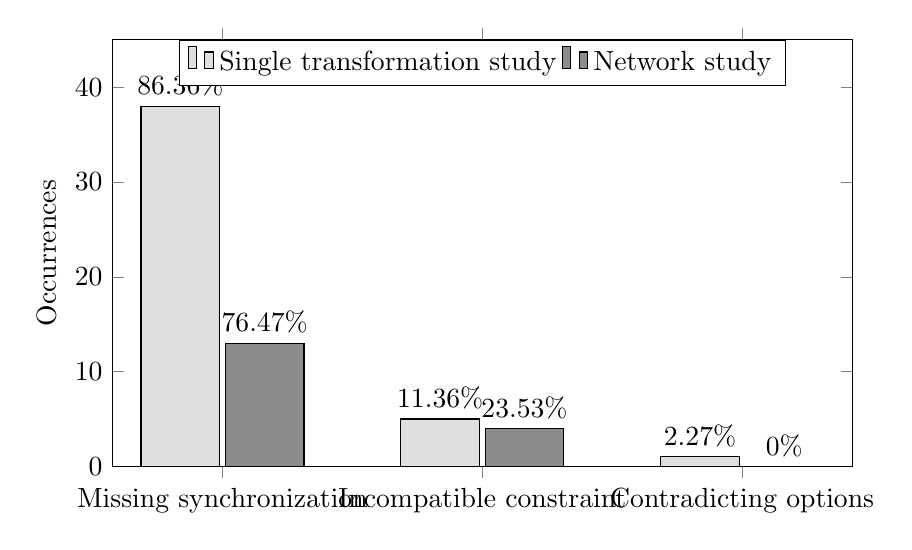
\begin{tikzpicture}
        \begin{axis}[
            ybar,
            bar width=1cm,
            x=3.3cm,
            height=7cm,
            legend style={at={(0.5,1)},anchor=north,legend columns=-1},
            ylabel={Occurrences},
            symbolic x coords={Missing synchronization, Incompatible constraint, Contradicting options},
            xtick=data,
            ymin=0,
            ymax=45,
            enlarge x limits={abs=1.4cm},
            nodes near coords align={vertical},
        ]
        \addplot[fill=gray!25,
            point meta={y*100/44}, % 44 Mistakes in total, calculate percentage
            nodes near coords={\pgfmathprintnumber\pgfplotspointmeta\%},
            ] table[x=Mistake type, y=both, col sep=comma] {
                Mistake type,              both
                Missing synchronization,   38
                Incompatible constraint,   5
                Contradicting options,     1
            };
        \addplot[fill=gray!90,
            point meta={y*100/17}, % 17 Mistakes in total, calculate percentage
            nodes near coords={\pgfmathprintnumber\pgfplotspointmeta\%},
            ] table[x=Mistake type, y=second, col sep=comma] {
                Mistake type,               second
                Missing synchronization,    13
                Incompatible constraint,    4
                Contradicting options,      0
            };
            \legend{Single transformation study, Network study}
        \end{axis}
    \end{tikzpicture}
    \caption[Number of occurrences of mistake types]{Absolute and relative number of occurrences of different mistake types in both case studies.}
    \label{fig:correctness_evaluation:errors:mistake_type_numbers}
\end{figure}

Relevance: Most relevant is synchronization, then compatibility, option selection occurred seldom and not other problems in case study
Although no option selection mistake in different, larger study, there was one in the first, only considering bidirectional transformations. Thus, we can expect this to be relevant for networks as well, even if it did not occur in the case study.
In answer to \autoref{eq:categorization:relevance}, we can see that missing synchronization is the most relevant mistake type, followed by incompatibilities.


\subsubsection{Orchestration}

Since we were able to categorize all occurring mistakes as consequences of actual mistakes that could have been avoided by proper construction or by analysis of the transformation, according to the identified mistakes types, and since all failures could be avoided when fixing the implementation faults as consequence of the mistakes, the transformation network was able to process all tested changed.
In consequence, the simple orchestration strategy was able to find consistent orchestrations in all cases.

In particular, if we consider that the strategy was very simple and was still able to find consistent orchestrations, at least in this case study the orchestration problem is not problematic.
In fact, the fail ratio we wanted to consider to evaluate how often the algorithm fails because of the orchestration problem in \autoref{eq:orchestration:relevance} is zero.


\subsubsection{Synchronization}

As discussed before, at transformation level 13 mistakes were made of only considering the network study and in total 51 mistakes were made when considering both studies.
They led to, in total, 211 failures.
All of them were fixed by adding matching of existing elements by explicit or implicit unique information, as proposed in \autoref{chap:synchronization:achieving:identification}.
This indicates that our approach is correct, as it fulfills the proposed property of resolving failures due to mistakes at the \leveltransformation level.
In fact, the success ratio metrics used to measure the correctness of our synchronization approach according to \autoref{eq:synchronization:correctness} is $1$, because for all considered changes that led to failures because of \leveltransformation level mistakes, consistency could be preserved after applying the approach.

Additionally, this shows that our approach could be applied in all cases in which failures occurred due to missing synchronization.
Thus, there were no cases in which the approach could not be applied.
This means that there were no cases in which no unique matching of elements could be performed.
Additionally, there were no failures due to missing synchronization that occurred for other reasons than missing element matching.
The application ratio to measure the applicability of our approach according to \autoref{eq:synchronization:applicability} is $1$.


\subsection{Topology Effects}

We consider the network case study. We counted the mistakes identified by occurring failures over the phases of adding single transformations.
We also considered incorrectness of the transformations.

\begin{table}
    \centering
    \small
    \renewcommand{\arraystretch}{1.5}
    \rowcolors{2}{gray!10}{}
    \begin{tabular}{L{9em}C{4.4em}C{4.4em}C{4.4em}C{4.4em}}
        \toprule
        \hspace{4.5em} \textbf{Phase $\rightarrow$} \newline \hspace{5.5em} \newline \textbf{$\downarrow$ Mistake Type} & 
        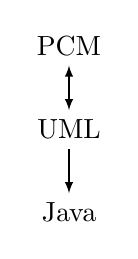
\begin{tikzpicture}
            \node[anchor=center] at (0,3em) (pcm) {PCM};
            \node[anchor=center] at (0,0em) (uml) {UML};
            \node[anchor=center] at (0,-3em) (java) {Java};
            \draw[latex-latex] (pcm) -- (uml);
            \draw[-latex] (uml) -- (java);
        \end{tikzpicture} & 
        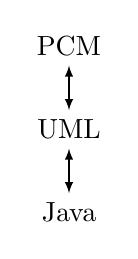
\begin{tikzpicture}
            \node[anchor=center] at (0,3em) (pcm) {PCM};
            \node[anchor=center] at (0,0em) (uml) {UML};
            \node[anchor=center] at (0,-3em) (java) {Java};
            \draw[latex-latex] (pcm) -- (uml);
            \draw[latex-latex] (uml) -- (java);
        \end{tikzpicture} & 
        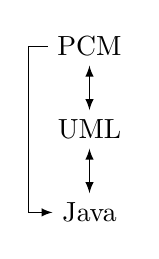
\begin{tikzpicture}
            \node[anchor=center] at (0,3em) (pcm) {PCM};
            \node[anchor=center] at (0,0em) (uml) {UML};
            \node[anchor=center] at (0,-3em) (java) {Java};
            \draw[latex-latex] (pcm) -- (uml);
            \draw[latex-latex] (uml) -- (java);
            \draw[-latex] (pcm.west) -- ++(-0.7em,0) |- (java);
            %\draw[-latex] (pcm.north) |- ++(-2em,0.7em) |- ([yshift=-0.7em]java.south) -- (java);
        \end{tikzpicture} & 
        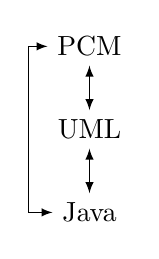
\begin{tikzpicture}
            \node[anchor=center] at (0,3em) (pcm) {PCM};
            \node[anchor=center] at (0,0em) (uml) {UML};
            \node[anchor=center] at (0,-3em) (java) {Java};
            \draw[latex-latex] (pcm) -- (uml);
            \draw[latex-latex] (uml) -- (java);
            \draw[latex-latex] (pcm.west) -- ++(-0.7em,0) |- (java);
        \end{tikzpicture}\\
        \midrule
        Transformation Incorrectness & 5 & 2 & 4 & 1 \\
        Missing Synchronization     & 0 & 0 & 6 & 7 \\
        Incompatible Constraints  & 0 & 0 & 2 & 2 \\
        Incompatible \newline Option Selection & 0 & 0 & 0 & 0 \\
        \bottomrule
    \end{tabular}
    \caption[Mistake types by case study phase]{Number of occurrences of different mistake types by the phase of the network case study with the stepwise addition of unidirectional transformations.}
    \label{tab:correctness_evaluation:errors:mistakes_by_phase}
\end{table}

The expected result is that synchronization mistakes first occurred when a cycle of the unidirectional transformations occurs which does not only consist of the cycle within one bidirectional transformations.
Only in that setting a synchronization scenario occurs which requires transformations to consider that other transformations may have created elements in both models.
Additionally, also errors at the network levels only occurred in those stages, although they could already occur in a linear network, like they also occurred in the single transformation case study, in which already the unidirectional consistency relations could be incompatible.



We had to perform two iterations of the previously described process.
In the first iteration, we faced failures due to mistakes at the operationalization level, whereas in the second iteration only failures due to remaining mistakes at the modularization level occurred.
We have tagged the states before and after the evaluation process in the GitHub repository~\cite{vitruvCBSEGithub}.

%\compactsubsection{Classification}

In the first iteration, all 187 tests failed.
The reason was that all transformations assumed that new elements are only created by the user or the transformation itself.
In consequence, we observed multiple instantiations and insertions in 187 cases, which we could trace back to 35 missing matchings of elements in the transformations.
After adding appropriate matchings, all these failures disappeared in a second iteration, so for the first iteration $\mathit{identifiedFailureRatio = resolvedFailureRatio = 1}$, since all detected failures were identified and resolved.

In the second iteration, 5 new failures occurred.
Three of them were diverging loops, which were caused by a namespace repeatedly prefixed to the name of classes, interfaces and enumerations in Java.
The causing mistakes were incompatible constraints: The Java model contains the fully qualified name of a class, whereas the UML model only contains the simple name, which was correctly propagated from UML to Java, but the namespace prefix was not removed in the opposite direction.
The two other failures were alternating loops, which were caused by alternations of element visibilities.
For methods and constructors, the visibilities were repeatedly changed due to an inconsistent mapping of visibilities from UML to Java and vice versa.
%After fixing the mistakes, two failures remained.
%Nevertheless, the reason for that were technical issues with the transformation engine due to its propagation of atomic changes.
%Since the original failures also disappeared in this case, we again have $identifiedFailureRatio = resolvedFailureRatio = 1$, since all detected failures were identified and resolved.
After fixing those mistakes, no failures remained.
So we again have $\mathit{identifiedFailureRatio = resolvedFailureRatio = 1}$, since all detected failures were identified and resolved. 

Summarizing, we were able to classify and resolve all failures in the case study and trace them back to mistakes with our classification in \autoref{chap:errors}.
This demonstrates the applicability of our categorization and is an indicator for the completeness and correctness of our catalog.
Most important, we did not find any failures that were caused by mistakes at a different specification level than we expected.
To further validate the catalog, we should apply it to further case studies.
It is however hard to find existing, independently developed transformations between at least three metamodels.
They would have to be developed in a schema similar to the one proposed by \textcite{kramer2016c}.
%\todoHeiko{Irgendwie noch sagen, dass wegen das wegen dem hohen Aufwand kein Threat to Validity ist? Oder kommt das nicht gut an?}
%\todoHeiko{Generell mehr Threats to Validity diskutieren?}


\todo{Erkennntis aus Iterationen: Solange wir nur einen Baum von Relationen haben, gibt es keine Fehler auf Modularisierungsebene (keine Inkompatibilitäten), diese kommen erst bei Zyklus hinzu (allerdings schon bei internem Zyklus durch Unidirektionalität?). D.h. wie schon voher angegeben sind Inkompatibilitäten per Konstruktion vermieden, wenn wir nur einen Baum von Relationen haben.
Falls wir keinen Baum garantieren können: In this case, the consistency specifications must be revised whenever non-termination or non-deterministic termination of consistency preservation is observed (see \autoref{fig:correctness:categorization})}


%\compactsubsection{Element Matching}

%In \autoref{sec:avoiding:matching}, we presented three levels of matching equal elements across different transformation paths.
%We used our case study to investigate, which of those levels are necessary in a practical scenario.

\end{copiedFrom} % ICMT


\subsection{Discussion}

Erkenntnis: Immer erst Fehler auf Transformationsebene fixen, da diese Fehler auf den anderen Ebenen verdecken.

Erkenntnis: Was wir nicht ausschließen können sind Fehler in den Konsistenzrelationen, die auf der unterschiedlichen Interpretation von Konsistenz basieren. Wenn beispielsweise die Relation UML<>PCM das Repo klein schreibt, Java<>PCM aber das Repo groß schreibt, wird das (korrekterweise) nicht gemacht.
Hier ist eine andere Auffassung von Korrektheit verletzt (Korrektheit der modularen bzgl. einer einheitlichen globalen Spezifikation), da implizit vorausgesetzt wird, dass in einem globale Verständnis in beiden Fällen auf das gleiche Repository abgebildet wird. (siehe Figure 6.4 in MA Timur).
Dies war explizit nicht die Art von Korrektheit die wir betrachtet haben, da sie ein anderes Ziel verfolgt. Sie erfordert Kenntnis über die übergeordnete Semantik der Elemente, beispielsweise durch eine globale Konsistenzspezifikation, gegen die man das prüft (siehe entsprechendes Kapitel) oder durch die Abbildung auf einen gemeinsamen Formalismus, der verifizierbar ist.

In Timurs MA außerdem betrachtet wie sich eine Kategorisierung in too many, incorrect and too few elements auf failures auswirkt. Hieraus konnten jedoch keine relevanten Erkenntnisse gezogen werden, weshalb wir es hier nicht diskutieren und auf die MA verweisen (Table 5.2)


\subsubsection{Threats to Validity}
- The transformation were not constructed synchronizing, thus obviously many synchronization errors occur. If the scenario is foreseen, there may be much less errors at this level and more at the others -> need to perform further evaluation were developer know about necessity to use transformations in a network to properly construct them and then see how often that still fails. (future work)


\paragraph{User Interaction}
Erlaubt Java->PCM, dass man an beliebiger Stelle ein Interface anlegen kann. PCM-UML erlaubt das nur im contracts-Package. Erstellt man ein Interface in einem anderen Package, erstellt PCM-UML nochmal eines im contracts Package, dadurch auch UML-Java und dann matcht UML-PCM, wodurch es bei PCM-Java zwei Abbildungen des Interface gibt. Hier haben wir inkompatible Constraints, aber wenn die Nutzerabfrage für das Matching in beiden Transformationen PCM-Java und PCM-UML eingebaut wird, kann der Nutzer konfligierende Entscheidungen treffen. Um das zu verhindern, müssten die Transformationen aufeinander abgestimmt werden.

Generell: Nutzerinteraktion lässt sich bei den Relationen dadurch ausdrücken, dass alle Auswahloptionen als valide consistency relation pairs betrachtet werden.
Problematisch sind jedoch die consistency preservation rules, da sie es potentiell erlauben konfligierende der condition elements auszuwählen, genauso wie es bei den Transformationen selbst auch passieren kann.
Wir haben diese selection of options im Orchestrierungs-Kapitel diskutiert.
Hier ist definitiv noch Future Work notwendig um zu untersuchen, wie man Nutzerentscheidungen über mehrere Transformationen hinweg miteinander alignen kann \todo{Future Work}.
Generell ist eine Untersuchung des Alignments von CPRs sinnvolles \todo{Future Work}.


\subsubsection{Limitations}
